% Vorlage für eine Bachelorarbeit
% Siehe auch LaTeX-Kurs von Mathematik-Online
% www.mathematik-online.org/kurse
% Anpassungen für die Fakultät für Mathematik
% am KIT durch Klaus Spitzmüller und Roland Schnaubelt im Dezember 2011

\documentclass[12pt,a4paper,titlepage,headinclude,bibtotoc]{scrartcl}
% scrartcl ist eine abgeleitete Artikel-Klasse im Koma-Skript
% zur Kontrolle des Umbruchs Klassenoption draft verwenden



% die folgenden Packete erlauben den Gebrauch von Umlauten und ß
% in der Latex Datei
\usepackage[utf8]{inputenc}
% \usepackage[latin1]{inputenc} %  Alternativ unter Windows
\usepackage{scrpage2}
\pagestyle{scrheadings}
\usepackage{comment}
\usepackage[T1]{fontenc}
\usepackage[english]{babel}
\usepackage{siunitx}
\usepackage{float}
\usepackage{chngcntr}
\usepackage{bm}
\counterwithin{figure}{section}

\usepackage[pdftex]{graphicx}
\usepackage{latexsym}
\usepackage{amsmath,amssymb,amsthm}
\usepackage{hyperref}
\usepackage{caption}
\usepackage{subcaption}
% Abstand obere Blattkante zur Kopfzeile ist 2.54cm - 15mm
\setlength{\topmargin}{-15mm}


% Umgebungen für Definitionen, Sätze, usw.
% Es werden Sätze, Definitionen etc innerhalb einer Section mit
% 1.1, 1.2 etc durchnummeriert, ebenso die Gleichungen mit (1.1), (1.2) ..

\newtheorem{Satz}{Satz}[section]
\newtheorem{Definition}[Satz]{Definition}     
\newtheorem{Lemma}[Satz]{Lemma}	
                  
\numberwithin{equation}{section} 

% einige Abkuerzungen
\newcommand{\C}{\mathbb{C}} % komplexe
\newcommand{\K}{\mathbb{K}} % komplexe
\newcommand{\R}{\mathbb{R}} % reelle
\newcommand{\Q}{\mathbb{Q}} % rationale
\newcommand{\Z}{\mathbb{Z}} % ganze
\newcommand{\N}{\mathbb{N}} % natuerliche



\begin{document}
  % Keine Seitenzahlen im Vorspann

  % Titelblatt der Arbeit
  \begin{titlepage}


    \vspace*{2cm} 

 \begin{center} \large 
    
    Master thesis\\
    \vspace*{2cm}
    {\huge LLLLLl\\}
    \vspace*{1.5cm}
   {\huge LLLLL}\\
   
    \vspace*{1.5cm}
	prepared by\\
	\vspace*{1cm}
   \textbf{\Large Johannes Riebold}\\
   \vspace*{1cm}
   from Schelldorf\\
   \vspace{2cm}
    \end{center}
    \begin{tabbing}
   \vspace*{1cm}
  \= \textbf{ Date of submission:}\= 55.5\\
   \vspace{0.8cm}
   \> \textbf{ First referee:} \>  \\
    \vspace*{0.3cm}
   \> \textbf{ Second referee:} \> 
    \end{tabbing}


    
    
 
\end{titlepage}
\newpage
\section*{Abstract}

\newpage
  % Inhaltsverzeichnis
  \tableofcontents

\newpage

  % Ab sofort Seitenzahlen in der Kopfzeile anzeveigen
  



\newpage
  





\section{Introduction}
\label{sec:Einleitung}

\section{Foundations}
\subsection{Teleconnections}
\label{sub:tele}
It has long been recognised that global atmospheric weather systems are linked on intraannual and longer timescales, which was first noted and recorded in David Crantz’s
\textit{The History of Greenland(1767):\\
“It has been many times remarked, that the weather in Greenland is just the reverse to that in Europe; so that when the temperate climates are incommoded with a very hard winter, it is here uncommonly mild, and vice versa”.}\cite{Kidston2009}\\

In the 1920s, more extensive studies on atmospheric linkages and oscillations were carried out by Sir Gilbert Walker. Three patterns of pressure anomalies were noted and named the \textit{North Atlantic Oscillation} (NAO), \textit{North Pacific Oscillation} (NPO) and \textit{Southern Oscillation}. The latter SO relates to a see-saw like oscillation of sea level pressure in different sectors of the Pacific Ocean named the Walker circulation in his honour many years later, which is closely related to the well known El Nino Southern Oscillation (ENSO) \cite{Gong1999} \cite{WALKER1923}. \\

In this connection, the term teleconnection in atmospheric science is commonly used to describe climatic linkages, either directly or indirectly, between geographically separated regions, which might be thousands of kilometres apart from each other. The word teleconnection was first used in the mid 1930s \cite{Angstrom1935} and has not established itself in climatic literature  until the 1980s. Generally, these linkages can proceed on interannual?? as well as on decadal time scales and are mostly associated with oscillations. Any phenomena that shows fluctuations around a mean value in some kind of periodic way is named an oscillation. 
 In atmospheric science, these anomalies  could principally emerge in all possible kinds of climatic variables, such as sea surface temperatures, zonal winds,  pressure fields etcetera(etc.). The terms anomaly and fluctuation are thereby associated with the deviation of the climatic field from its respective mean annual cycle.
 
  Thus, teleconnections are commonly characterised by simultaneous fluctuations of a climatic field of opposite or even the same sign within separated areas. The name basically refers to the fact that these either positive or negative correlations suggest, that some kind of information is transported between the distant regions throughout the atmosphere. By employing statistical analysis techniques, such as correlation and regression maps or empirical orthogonal function analysis, on  observed interannual??? and decadal?? variability of sea level pressure, zonal wind or geopotential height fields, these teleconnection patterns can be identified[????].\\
It shows up, that these patterns occur around the globe, as well on the northern hemisphere as well as on the southern hemisphere....\\\\


 






	\subsection{AO}


	\subsubsection{Southern Annular Mode (SAM)}
	The question is, whether there are other oscillations like SO,NAO,NPO????
	In 1928, Sir Gilbert Walker stated: \textit{Just as in the North Atlantic there is a pressure opposition between the Azores and Iceland,... ,there is an opposition between the high pressure belt across Chile and the Argentine on the one hand, and the low pressure area of Weddell Sea and the Bellingshausen Sea on the other} \cite{Gong1999}
	However, the scarcity of observational data about this region did not allow for more profound research on this supposed oscillation. \\
	In the 1980s, when more data about the Southern Hemisphere became available and more analyses were carried out, the existence of such an oscillation in the mid and high southern latitudes was confirmed and named the \textit{Antarctic Oscillation} (AO) [??].
	The Antarctic Oscillation, also known as the Southern Annular Mode (SAM), describes the most dominant mode of extratropical climate variability on timescales ranging from interannual to intraseasonal timescales over the Southern Hemisphere \cite{Thompson2000}. By convention, it is associated with an alternation of masses between the mid and the high latitudes resulting in higher pressure anomalies over the mid-latitudes and lower pressure anomalies over Antarctica in its positive phase and vice versa in its negative phase. For illustration, figure \ref{fig:SAM_low_high} shows polarstereographic plots of the ERA-Interim monthly geopotential height anomalies for a  negative phase (February 2002) and a positive phase (May 1989). 

\begin{figure}
		\centering
		\includegraphics[scale=0.4]{pictures/SAM_low_high.png}
		\caption{left February 2002 right May1989}\label{fig:SAM_low_high}
		
\end{figure}	
	
	
	
	Furthermore,figure \ref{fig:correlation_sam} depicts the crosscorrelation coefficients of monthly zonally averaged geopotential height anomalies of the 700\,hPa pressure level in the Southern Hemisphere using ERA-Interim reanalysis data. The SAM manifests itself in the strong and significant negative correlation down to -0.76 between the midlatitudes (40$^\circ$S) and the high-latitudes(60-70$^\circ$S) \cite{Gong1999}, which implies that increasing pressures above the mid-latitudes are typically accompanied by decreasing pressures above the high latitudes and vice versa.\\
	For characterising the current state of the SAM in a respective month several SAM-indices have been defined over time. The first and maybe most simplest definition of a SAM index (SAMI) using reanalysis data was given by Gong and Wang (1999) \cite{Gong1999}:
	\begin{align}\label{eq:Gong}
		\text{SAMI}=P^{*}_{40^\circ S}-P^{*}_{65^\circ S},
	\end{align}
where $P^{*}_{40^\circ S}$ and $P^{*}_{65^\circ S}$ stands for the normalised zonal mean SLP of 40$^\circ$S and 65$^\circ$S for every month respectively. A slightly different definition is given by Nan and Li (2003) \cite{Nan2003}, who used 70$^\circ$S zonal mean SLP  $P^{*}_{70^\circ S}$ instead of  $P^{*}_{65^\circ S}$ by reason of supposedly stronger negative correlations in the zonally-mean? SLP between 40$^\circ$S and 70$^\circ$S compared to 40$^\circ$S and 65$^\circ$S. In order to examine the reliability of such reanalysis-based SAMI before the satellite era, station based indices have been introduced, for instance by  Marshall \cite{Marshall2003}, who uses mean SLP observations from six stations located at 40$^\circ$S and 65$^\circ$S respectively to provide a proxy zonal mean.\\
A more sophisticated and commonly used definition of the SAMI is given by the first principal component of the Leading Empirical Orthogonal Function as described in chapter \ref{subsec:EOF}. Many more indices with their individual strengths and weaknesses have been defined over the last years and it also points out that time series of differently defined SAMI are strongly and significantly correlated with each other.\cite{Ho2012a}\\

To get a notion of the coarse shape of the SAM, Figure \ref{fig:ind_mslp_regress} illustrates a linear regression of the time series of monthly zonal mean ERA-Interim geopotential height anomaly fields onto the standardized  time  series of monthly SAMI calculated according to equation \ref{eq:Gong} for the NOAA 20th-Century Reanalysis data [taken fromwebsite, oder lieber IERA ???]. Apparently, an increase of the SAMI by its standard deviation is typically accompanied by a decrease of the 700\,hPa height level of more than 20\,gpm over the entire Antarctic continent down to 50\,gpm over the Amundsen sea in western Antarctica, whereas over the mid-latitudes an overall increase with maxima up to 30\,gpm over the three oceans can be observed. Thus, despite the fact that the term "annular"  suggests that the SAM occurs in a zonally? symmetric and ring-shaped pattern, a strong nonsymmetric wave-3-pattern over the mid-latitudes is detectable, which is presumably closely connected to planetary Rossby-waves.  Fogt ....
As model studies suggested the SAM owes its existence to internal atmospheric dynamics



	
\subsubsection{Impacts on Southern Hemisphere('s) Climate}
Several studies have demonstrated that the SAM has an important and significant influence on the climate system over the entire southern hemisphere[???].\\
 Due to an increase of the meridional pressure gradient  $\frac{\partial p}{\partial y}$ between the mid and the high-latitudes, a positive SAM phase is associated with a strengthening of the westerly wind belt. This fact can be explained by considering the geostrophic equation
\begin{align*}
	fu=\frac{1}{\rho}\frac{\partial p}{\partial y},
\end{align*}
which describes the proportional relationship between the zonal wind speed $u$ and the meridional pressure gradient $\frac{\partial p}{\partial y}$ for a frictionless fluid on a rotating sphere with the hydrostatic and steady state approximation being made. The parameter $f$ describes the coriolis parameter and $\rho$  the air density.\\
 A regressions  between the SAM index and wind speed wind direction \cite{Lovenduski2005}, as done in figure \ref{dd}, indicates that the anomalously strong pressure gradient during  a positive SAMI acts to significantly strengthen the westerly winds at around 55$^\circ$S, and to weaken the westerlies at around 35$^\circ$S (easterly anomaly), by \SI{0.9}{\metre\per\second} in certain regions, resulting in a shift of the westerly wind belt towards Antarctica. In this connection, a southward shift of the Antarctic circumpolar stormtrack has been recognised \cite{Thompson2000},\cite{Gillett2006}, which acts as a relatively narrow zone, in which extratropical cyclonic storms travel driven by the prevailing winds. It has been shown that these  changes in atmospheric circulation impact other components of the climate system in the Southern Hemisphere as well\cite{Hall2002}.\\
 
It has been shown, that the frictional transfer of momentum at the air–sea interface has affects ocean circulation in the southern hemisphere. Westerly wind anomalies in the positive SAM phase increase northward Eckman transport of surface water between 45$^\circ$S and 65$^\circ$S and easterly wind anomalies induce stronger southward Eckman transport between 30$^\circ$S and 45$^\circ$S. Mass conservation induces that the divergence around the Antarctic coast implies stronger warm and nutrient-rich deep water upwelling, which favours biological productivity, whereas the convergence around 45$^\circ$S causes  stronger surface water downwelling \cite{Lovenduski2005}. Figure \ref{qq} depicts the regression between the SAMI and chlorophyll concentration and indicates a strengthening around the Antarctic coast of production as a response to increasing SAMI and( a weakening around 45$^\circ$S).  Additionally, a more intense circumpolar current may be associated with an increasing SAMI \cite{Hall2002}\\

Analyses about the effect of an increasing SAMI on the sea-ice extend in the Southern ocean suggest that the main response results in a decrease of ice in the Weddell Sea, and an increase in the Ross Sea, Amundsen Sea and parts of the Pacific sector \cite{Lefebvre2004}.\\

The previously described upwelling effect of  warm deep water around the Antarctic coast has shown to be connected to stronger ice shelf basin melt, which possibly acts as a driver for the destabilisation of the Antarctic Ice Shelf \cite{Greene2017}.
Other studies demonstrated that a positive SAM phase is associated with anomalously cold surface temperatures over most of Antarctica and warming over the Antarctic Peninsula. Furthermore, decrease in zonal SST in the circumpolar region, increases in the subtropics  \cite{Hall2002} and significant regional warmings over southern Chile and Argentina, over Tasmania and south- eastern Australia over the South Island of New Zealand have been observed in connection with a increasing SAMI \cite{Gillett2006}.\\

Additionally to the previous aspects, several other studies have been published about the SAM's influence on other earth system components, such as carbon cycle \cite{Butler2007} and precipitation over the Southern Hemisphere \cite{Silvestri2003}.





 
	
	
	\begin{figure}
		\centering
		\includegraphics[scale=0.4]{pictures/correlation_IERA.png}
		\caption{Crosscorrelation coefficients of zonal-averaged Sea Level Pressure (SLP) anomalies in the SH using} \label{fig:correlation_sam}
	\end{figure}
	
	\begin{figure}
		\includegraphics[scale=0.5]{pictures/regression_all.png}
		\caption{jj} 
	\end{figure}
	
%	\begin{figure}
%		\includegraphics[scale=0.5]{pictures/SAM_index_20CR.png}
%		\caption{(20 CR taken from \cite{Zheng2013a}} 
%	\end{figure}
%	
%	\begin{figure}
%		\includegraphics[scale=0.5]{pictures/SST_corr_SAMindex.png}
%		\caption{taken from \cite{Screen2009}}
%	\end{figure}
%	
%	\begin{figure}
%		\includegraphics[scale=0.5]{pictures/station_based_SAM}
%		\caption{taken from \cite{station_based_SAM}}
%	\end{figure}
	
	\begin{figure}
		\includegraphics[scale=0.75]{pictures/SAM_regression_SST_wind.png}
		\caption{taken from \cite{Lovenduski2005}}
	\end{figure}
	
	
	\subsection*{mechanism}
	\subsection{drivers of the sam}
	external forcings ozone greenhouse gas recovery
	evolution over millenia
\section{Methods}
\label{sec:Methods}


	
	\subsection{Empirical Orthogonal Function Analysis}
	\label{subsec:EOF}
	
Empirical Orthogonal Function (EOF) Analysis is a common and widely used statistical technique in atmospheric science for analysing data in high dimensional phase spaces.
The objective is to structure, to simplify  and especially to find in place of the ordinary original variables $x_i(t)$ a relatively small number of new independent variables $u_i(t)$  , which represent as much of the original data sets information as possible. For this reason, a new set of orthogonal coordinate axes $\bm{e_{i}^u}$ instead of the ordinary and often more intuitive axes $\bm{e_{i}^x}$ has to be found, in which to examine the data \cite{Wilks2006}??. 


Loosely speaking ,the desirable characteristics of the new orthogonal coordinate axis are given in such a way that:
\begin{itemize}
	\item the maximum possible amount of variance or variation within the data set can be explained along the 	axis $\bm{e_{1}^u}$ (with new coordinates $u_1(t)$)
	\item the maximum possible amount of remaining variance of the data set can be explained along the subsequent axis $\bm{e_{2}^u}$  
	\item and so forth for the remaining axis $\bm{e_{i}^u}$,
\end{itemize}
subjected to the condition, that the new variables $u_i(t)$ are uncorrelated with the variables having lower indices.\\
In contrast to other analysing and transformation techniques, such as Fourier Transforms or Taylor expansions, in which fixed sinusoidal or polynomial coordinate systems are used, the coordinate axes for an EOF analysis have to be identified uniquely for each specific data set.


		\subsubsection{Basic principle in two dimensions}
		\label{subsubsec:2d-case}
		
 The general procedure of EOF analysis can be best visualized and illustrated in the two dimensional case. For this reason, we will consider a two dimensional phase space with two variables $x_1$ and $x_2$ measured simultaneously at certain times, which for instance may be associated with two temperature measurements at two different locations. %As mentioned before, the main purpose of EOF analysis is to find a new set of %coordinate axes, which represent a large amount of variance of the data set.
In figure \ref{fig:EOF_2d}, the two variables $x_1$ and $x_2$ reveal a strong positive correlation. Instead of using the original coordinate system $\bm{e_{1}^x}$ and $\bm{e_{2}^x}$, which may be associated with the two variables $x_1$ and $x_2$, this system may be rotated for obtaining a new one with variables $u_1$ and $u_2$ and with new orthogonal coordinate axes $\bm{e_{1}^u}$ and $\bm{e_{2}^u}$. As depicted in figure \ref{fig:EOF_2d} (right), displaying the data set in the new $u$-coordinates shows, that most variance or spread of the data set is represented along the $\bm{e_{1}^u}$ axis. The remaining small amount of variance is explained along the orthogonal axes $\bm{e_{2}^u}$.\\
Thus it is obvious, that the initial 2-dimensional ??structure of the data set, can be reduced to a 1-dimensional perspective by just using the new variable $u_1$ , at the expanse of loosing a certain amount of information about the data set.

\begin{figure}
	\centering
		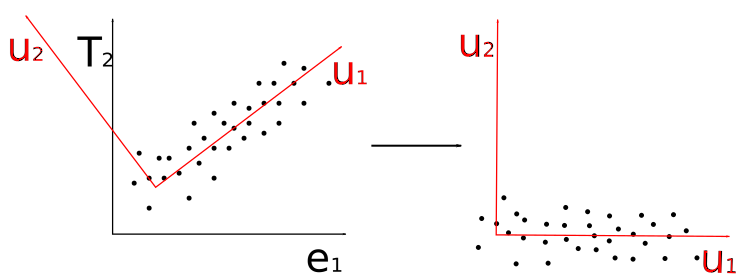
\includegraphics[scale=0.7]{pictures/EOF_2d}
		\caption{Illustration of the basic principle of an EOF analysis: A data set, which is initially represented in an intuitive $x$-coordinate system, may be examined in a new coordinate system with axes $\bm{e_{1}^u}$ and $\bm{e_{2}^u}$ and variables $u_1$ and $u_2$.....  } \label{fig:EOF_2d}
\end{figure}

		\subsubsection{Extension and Generalisation to higher dimensions}
EOF analysis reveals its greatest power, when it comes to analysing  high dimensional data sets, which are rather hard to visualize and structure due to the large number of necessary variables $x_i$.
For this reason, we will extend and generalise the previous considerations to higher N-dimensional phase spaces, which is the general case for a time series of climatic variables $x$ (e.g. sea surface temperature, pressure) defined on $N$ grid points around the globe and measured at $T$ different times $t_k$. (Thus we suppose, that $x$ is given at $N$ grid points at $T$ different time steps.) The climatic variable $x$ at a specific grid point $i=1,...,N$ at time $t_k$ ($k=1,2,...,T)$ is denoted by $x_i(t_k)$.
, which may be summarized at time $t_k$ in  vector notation as

\begin{align*}
	\bm{x(t_k)}=(x_0(t_k),x_1(t_k),...,x_N(t_k)).
\end{align*}
The original and most intuitive basis vectors are thus for instance given by $\bm{e_1^x}=(1,0,0,...,0)$, $\bm{e_2^x}=(0,1,0,...,0)$  with respective coordinates $x_1(t_k)$,$x_2(t_k)$ and so forth.
The objective is to find a new and unique coordinate system, which axes $\bm{e_i^u}$ are linear combinations of the originally defined axis $\bm{e_i^x}$ (i=1,...N) and which have the properties of explaining successively the most variance, as mentioned before in \ref{subsec:EOF}. The corresponding new time dependent variables $u_i(t_k)$ are related to the initial  basis vectors  $\bm{e_i^x}$  by the projection relation 
\begin{align*}\label{eq:projection}
u_i(t_k)=\bm{e_{i}^u} \bm{x}(t_k)= \sum\limits_{j=1}^N e_{ij}^u x_j(t_k). 
\end{align*}

In order to determine such a coordinate system $\bm{e_i^u}$, the covariance matrix $\bm{\underline{S}^x}$ of the $N$-dimensional time series $\bm{x}(t)$ has to be calculated, which components are defined as

\begin{align*}
	S^x_{ij}&=\text{E}[(x_i(t)-\mu_i)(x_j(t)-\mu_j)]\\
		&=\frac{1}{T} \sum\limits_{k=1}^T [(x_i(t_k)-\mu_i)(x_j(t_k)-\mu_j)]
\end{align*}

where $\mu_i$ denotes the time averaged expectation value at grid point $i$, which is given by

\begin{align*}
	\mu_i=\frac{1}{T}\sum\limits_{k=1}^Tx_i(t_k)	
\end{align*}

and the $x$-index signifies that the matrix is given in initial $x$ coordinates.

%The objective is to find a set of more complex basis vectors $e_i^u$ with respective %new coordinates $u_m$, which are related to the original simple basis vectors and %coordinates by the projection relation
%\begin{align*}
%u_m=\sum e_{mk}^u x_k e_{mk}^x 
%\end{align*}

It has been shown, that the desired new coordinate axes $\bm{e_i^u}$ are given by the eigenvectors of the covariance matrix $\bm{\underline{S}^x}$, which explain the highest possible amount of variance successively (cf. \ref{subsec:EOF}).
Since the covariance matrix $S_x$ is symmetric, its eigenvectors and thus the new coordinate axes $\bm{e_i^u}$ are orthogonal as required and its eigenvalues $\lambda_i$ are reel.
Transforming a symmetric matrix into a representation in its Eigenbasis always implies, that the result is a diagonal matrix. For this reason, the covariance matrix $\bm{\underline{S}^u}$ represented in the new coordinate system $\bm{e_i^u}$ (or Eigenbasis) has the shape

\[
\bm{\underline{S}^u}=
  \begin{pmatrix}
    \lambda_1 & 0 & \dots & 0 \\
    0 & \lambda_2 & \dots & 0 \\
    \vdots & \vdots & \ddots & \vdots \\
    0 & 0 & \dots & \lambda_N
  \end{pmatrix}
  .
\]
As the off-diagonal entries are zero, the new variables $u_i$, in which to represent the data and which are obtained according to equation \ref{eq:projection}, are uncorrelated with each other.\\
Furthermore, the respective reel valued eigenvalues $\lambda_i$ characterise the variance along the respective axis. The fraction of explained variance $\sigma_i^2$ along along an axis $\bm{e_{i}^u}$ is proportional to its respective eigenvalue $\lambda_i$ and given by the relation

\begin{align*}
	\sigma_i^2=\frac{\lambda_i}{\sum\limits_{j=1}^N \lambda_j}
\end{align*}


The new variables $u_i(t_k)$ are commonly called \textit{Principal Components} (PC) and the respective coordinate axes $\bm{e_{i}^u}$ are called \textit{Empirical Orthogonal Functions} (EOF).\\
Since vectors of different length, which are aligned into the same direction might act as eigenvectors of the correlation matrix $\bm{\underline{S}^x}$,there exist different scaling conventions for the EOFs and the corresponding PCs. For the following considerations(,) we will define the EOFs in such a way that the respective PC time series has unit variance.

		\subsection{Application to climatic data}
Since EOFs provide the most efficient set of orthogonal functions, in which to represent a given fraction of the variance of meteorological fields with a minimum number of coefficient (PCs), EOF analysis has been extensively used as an aid in climatological investigations and especially to identify the most dominant patterns of variability in the atmosphere \cite{Kidson1975}(Wallace and Gutzler 1981). For this reason, it has been shown that EOF analysis serves as a useful tool for identifying and characterising atmospheric oscillation and teleconnection patterns around the globe in many climatic variables \cite{Rogers1982} \cite{Thompson2000}??. Thus, 
For examining the structure and the temporal evolution of the SAM we use monthly geopotential height fields for specific pressure levels of the ERA-Interim reanalysis set between 20$^\circ$S and 88$^\circ$S and for the period 1979-2016. (As mentioned in ..) The horizontal resolution of the provided data is 1$^\circ$ along each latitudes and 1.77$^\circ$ along each longitude resulting in a phase space with 6300 dimensions. 
Since we are interested in deviation from the mean annual cycle
Due to the fact that grid points are equally spaced on a regular latitude-longitude grid, the number of grid points per unit area increases with higher latitudes(,)
as the meridians converge at the poles. Therefore, high latitude features would be amplified and mid latitude features deemphasized. In order to remedy this inhomogeneous spatial distribution of data points, a common approach is to multiply each grid by the square of the cosine of its respective latitude $\sqrt{\text{cos}(\varphi)}$.
The leading EOF
\begin{figure}
	\centering
	\includegraphics[scale=0.14]{pictures/EOF_PC_IERA.png}
	\caption{ggggggggggggggggggggggggggggggggggggg}\label{fig:eof_iera}
\end{figure}

\section{Data and models}
\subsection{ERA-Interim reanalysis Data}
For evaluating the performance of several climate models, data from ERA-Interim reanalysis are used for comparison, which is a global atmospheric reanalysis data set provided by  ECMWF (European  Centre  of  Medium-Range
Weather Forecasts) and the successor of the. The data set is continuously updated in real time and extends back to 1979. As with all reanalysis data, they are produced via data assimilation, a process that relies on both observational data (in-situ and satellite measurements) and model-based forecasts to estimate the true conditions of the climate system. The assimilation system used to produce the data includes a 4-dimensional variational analysis (with a 12-hour analysis window) and results in 6-hourly output with a spatial resolution of approximately 80 km (T255)????????? auflösung 1 mal 2 grad???? on 60 oder 37???? vertical levels from the surface up to $0.1,/$hPa.....\\\\
For our analysis we mostly use monthly averages of geopotential height fields of different pressure levels, measured in geopotential metres gpm (units $\frac{\mathrm{m}^2}{\mathrm{s}^2}$). A geopotential metre 1\,gpm corresponds to the height at which an air parcel with mass 1\,kg has a potential energy of 9.80665\,J.Thus, at mid-latitudes where the gravity constant $g$ is close to $g_0=9.80665\,\frac{\text{m}}{\mathrm{s}^2}$ a geopotential metre approximately coincides with the height of a geometric metre, whereas at the poles where $g>g_0$ a geopotential metre lies above the geometric height of 1\,m.?????? Since an air parcels moving  along a surface of constant geopotential heigth maintains its potential energy, the unit geopotential metre is commonly used in atmospheric research instead of geometric height $z$.
extrapolated bewlow 700 hPa
\subsection{models}
Climate
\subsubsection{MPI-ESM}
The Max Planck Institute - Earth System Model (MPI-ESM) is completely coupled climate model, which  couples the atmosphere, ocean and land surface through the exchange of energy, momentum, water and carbon dioxide. It is based on the following components:
\begin{description}

	\item ECHAM6??
		 is an atmospheric general circulation model, developed at the Max Planck Institute for Meteorology, which is based on a spectral-transform dynamical core. It is configured to run at different resolutions. For the Coupled Model Intercomparison Project 5 (CMIP5) ECHAM6.1 was used in the LR (T063L47) and MR (T063L95) resolution configurations, which stand for the truncation after the 63 wave component and 47 and 95 vertical levels respectively??
	\item MPIOM ( Max Planck Institute ocean model) is the primitive equation ocean sea-ice component of the MPI-ESM with hydrostatic and Boussinesq approximations made and computing on a C-grid.
	\item JSBACH is the land component of the MPI-ESM, which simulates biogeochemical and biogeophysical terrestrial processes and provides the lower boundary conditions for the atmospheric component over land 
	\item HAMOCC is a global ocean biogeochemistry model
\end{description}

The coupling of atmosphere and land on the one hand and ocean and biogeochemistry on the other hand is done by using the separate coupling program OASIS3.

\newpage
\bibliographystyle{unsrt}
\bibliography{Masterarbeit.bib}



\end{document}

